% \iffalse meta-comment
% (c) 2021 Vincent Kuhlmann
% 
% \fi
% \iffalse
%<*driver>
\ProvidesFile{highlightlatex.dtx}[2021/03/17 highlightlatex v1.0.0 + Dev]
\NeedsTeXFormat{LaTeX2e}[1994/06/01]
\documentclass{ltxdoc}

\usepackage[margin=2.54cm]{geometry}
\usepackage{graphicx}
\usepackage{parskip}
\usepackage{listings}
\usepackage{adjustbox}
\usepackage{soul}
\usepackage{hyperref}
\usepackage{xcolor}

\iftrue \iffalse Use own package\fi
    \usepackage{highlightlatex}
    \updatehighlight{
    	name = default,
    	add = {
    		\defaultgobble
	    },
    	name = hll,
    	color = orange!90!black,
    	add = {
    		\hll, highlightblock
    	},
    	name = vert,
    	color = red,
    	add = {
    		|	
	    }
	}   
\else
    \let\hll\lstinline
    \lstnewenvironment{highlightblock}[1][]
    {%
        \lstset{#1}%
    }{}%
    \lstset{tabsize=2,escapeinside=~~}
\fi
\colorlet{codeBackground}{gray!6!white}

\newcommand\fhref[2]{%
	\href{#1}{#2}\;\footnote{\,\url{#1}}\,%
}

\newlength\centerlabelledwidth
\newlength\centerlabelledminleft
\def\centerlabelledlabel{}
\setlength\centerlabelledminleft{5em}
\expandafter\newif\csname ifshowcasecenter\endcsname

\makeatletter
\define@key{centerlabelled}{label}{%
	\def\centerlabelledlabel{#1}%
}

\define@key{centerlabelled}{width}{%
	\setlength\centerlabelledwidth{\dimexpr #1\relax}%
}

\define@key{centerlabelled}{frac}{%
	\setlength\centerlabelledwidth{\dimexpr #1\textwidth\relax}%
}

\define@key{centerlabelled}{left}[]{%
	\showcasecenterfalse
}

\define@key{centerlabelled}{center}[]{%
	\showcasecentertrue
}

\define@key{centerlabelled}{minleft}{%
	\setlength\centerlabelledminleft{#1}%
}
\makeatother

\newlength\showcaseleft

\newenvironment{centerlabelled}[1][]{%
	\setlength\centerlabelledwidth{\textwidth}%
	\setkeys{centerlabelled}{#1}%
	\setlength\showcaseleft{\dimexpr(\textwidth-\centerlabelledwidth)/2\relax}%
	\ifshowcasecenter
		\ifdim\centerlabelledminleft>\showcaseleft\relax
			\showcasecenterfalse
		\fi
	\fi
	%
	\unless\ifshowcasecenter
		\setlength\showcaseleft\centerlabelledminleft
		\ifdim\dimexpr\textwidth-\centerlabelledminleft\relax<\centerlabelledwidth\relax
			\setlength\centerlabelledwidth{\dimexpr\textwidth-\centerlabelledminleft\relax}%
		\fi
	\fi
	%
	\par\penalty 10000%
	\hspace{\showcaseleft}%
	\adjustbox{raise=-6pt,lap=-\width-0.7em}{\setulcolor{red}\expandafter\ul\expandafter{\expandafter\textsc\expandafter{\centerlabelledlabel}}}%
	\begin{minipage}[t]{\centerlabelledwidth}%
}{%
	\end{minipage}%
}

\newenvironment{showcase}{%
	\begin{centerlabelled}%
}
{%
	\end{centerlabelled}
}

\begin{document}
    \DocInput{\jobname.dtx}
\end{document}
%</driver>
% \fi
%
% \newbox\cmdintitle
% \setbox\cmdintitle=\hbox{\hll|highlightlatex|}%
% \setbox\cmdintitle=\hbox{\adjustbox{height=2.0\height}{\usebox\cmdintitle}}
% 
% \title{\vspace{-2cm}Package \usebox\cmdintitle{} manual}
% \author{%
%    Vincent Kuhlmann\\
%     \texttt{vincent.kuhlmann@hotmail.com}
% }
%
%
% \maketitle
% \begin{abstract}
%
% This package provides colored syntax highlighting for \LaTeX{} source code,
% without aid from outside \LaTeX. This is in response to the general trend that people often fall back to verbatim for displaying code. This package aims to make good looking \LaTeX{} source code feasible for all users. For this, it
% builds further on the generic `listings' package. A possible output is shown in \autoref{fig:demoOutput}\,.

% \end{abstract}
% 
% \tableofcontents
% 
% %\vfil
%
% \begin{figure}[htbp]
%     \centering
%     \rule{2cm}{1pt}
%
%     \medskip
%     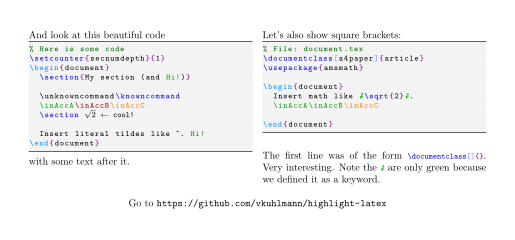
\includegraphics[width=0.9\textwidth,trim=1cm 1cm 1cm 1cm, clip]{demo.pdf}
%     \caption{Output of `demo.tex'.}\label{fig:demoOutput}
%     \rule{2cm}{1pt}
% \end{figure}
% 
% \iffalse
% \begin{macro}{\mymacro}
%     someTest
% \end{macro}

% \DescribeEnv{myenv}
% aaa
% \fi
% 
% \section{Getting started}
% 
% After having added the package, you can add LaTeX in two ways.
% 
% \subsection{Inline style}%
%
% \begin{showcase}[label=example]%
%   \begin{highlightblock}[gobble=6]
%      Your file begins with a line of the form \hll~{}~|\documentclass[]{}|. The
%      square brackets ...
%   \end{highlightblock}%
% \end{showcase}
% 
% The first non-space character following \lstinline|\hll| delimits the argument to
% this command.
% 
% \subsection{Block style}
% 
%
% \begin{showcase}[label=example]
% \begin{highlightblock}[gobble=5]
%     Your basic document now looks like
%     \begin{highlightblock}[gobble=2]
%       \documentclass[a4paper]{article}
%       \begin{document}
%          Hello world!
%       \end{document}
%     \end{~{}~highlightblock}
% \end{highlightblock}
% \end{showcase}
% 
% To prevent indentation of our \hll|highlightblock| (here one tab) to be shown
% as part of the code, the \hll|gobble| parameter strips them off. Play around
% with it until everything looks right. I recommend to set this value globally
% using \hll|\def\defaultgobble{2}|. You can still override it on a per-block
% basis, if necessary.
%
% There are situations where width of the block could run out of the page. For
% example, when using beamer and storing a block as described in the section
% `Fragile breaking situations', the normal full-width of a slide is assumed. If
% you use multiple columns, set the \hll|linewidth| on the \hll|highlightblock|.
% This can be a fraction of the total slide width available, \hll|0.6\textwidth|
% is 60\% of the width, or an absolute value, like \hll|10em|, which seems to
% equal 20 characters.
%

%
% There are more keys you can provide. Check the
% \fhref{https://www.ctan.org/pkg/listings}{\hll|listings| package
% documentation} for options
% available to the \hll|lstlisting|-environment and \hll|lstset| command.
%
% \newbox\uphbox
% \setbox\uphbox=\hbox{\hll|\updatehighlight|}%
% \setbox\uphbox=\hbox{\adjustbox{height=1.4\height}{\usebox\uphbox}}
%
% \section[Macro \textbackslash updatehighlight]{Macro \texorpdfstring{\usebox\uphbox}{\textbackslash updatehighlight}}
% \subsection{Adding a command to a highlighting rule}
%
% By default, only some LaTeX commands will be highlighted in blue. If there are
% others you need, like \hll|\tableofcontents| and \hll|\figref|, update the
% highlighting rules:
% \begin{showcase}[label=use]
%     \begin{highlightblock}[gobble=9]
%         \updatehighlight{
%           name = default,
%           add = {
%             \tableofcontents, \figref
%           }
%         }
%     \end{highlightblock}
% \end{showcase}
% 
% The change will only affect code after it. I recommend issuing
% \hll|updatehighlight| in your preamble (before the \hll|\begin{document}|). In
% some situations you might want to change things mid-document. That's possible
% too.
%
% \subsection{Custom highlighting rules}
% \subsubsection{Example}
%
% As shown in \hll|demo.tex|, you can put any command or keyword you want to
% highlight in a different color. You do this with
% \begin{showcase}[label=example]
%	  \begin{highlightblock}[gobble=9]
%         \updatehighlight{
%           % name: How you like to refer to it. Allows you to modify the style later.
%           name = spotlight,
%           color = orange,
%           add = {
%               \tableofcontents
%           }
%         }
%     \end{highlightblock}
% \end{showcase}
%     
% You can use the \hll|xcolor| syntax for describing colors as well. If you find the
% orange too bright, you can replace it with \hll|orange!90!black|: 90\% orange,
% remaining is black. For more information on color definitions and name, refer
% to \fhref{https://en.wikibooks.org/wiki/LaTeX/Colors}{LaTeX/Colors on Wikibooks}.
%
% \iffalse\medskip\rule{5cm}{0.4pt}\medskip\fi
%
% \subsubsection{Specification}
%
% The argument to \hll|\updatehighlight| is a key-value list. Keys are processed
% sequentially. For example, use \hll|color| before \hll|add| rather than after it, and
% a key can appear multiple times. Each one will be processed. You can merge any
% two \hll|\updatehighlight| in one. No need to close and reopen \hll|\updatehighlight|
% for each highlighting rule.
%
% You might be tempted to add a blank line for clarity; that means a new
% paragraph to LaTeX, don't do it. Instead, just put a line with only a \hll|\%|
% sign. Spacing within the argument is often irrelevant. If you need a comma in
% the value, surround your value with braces.
%
% \iffalse The possible keys are:
% \begin{itemize}
% 	\item[\textbf{name}.] 
% 	
%	\item[\textbf{classoffset}.] Set the \hll|listings| classoffset manually. Try to avoid this.
%   Use \textbf{name} to refer to existing rules instead.
%
%   \item[\textbf{add}.] Add a commands (\hll|\mycommand|) or keyword (\hll|Hi!|) to the current
%   rule. The value can contain multiple values by opening braces, and comma
%   separating values within them.
%
% \end{itemize}\fi

% \begin{list}{}{%
%     \itemindent-\leftmargin%
%	  \setlength{\itemsep}{10pt}%
% }
%	\item\textbf{name}\par\nobreak
%
%	Creates or modifies a named rule. This key is optional.
% 	
% 	The default keys are \hll|default|, which includes a bunch of basic commands, and
% 	has by default a dark blue color, and \hll|structure|, which consists of \hll|\begin|
% 	and \hll|\end| and prints them in light blue.
%
%
%	\item\textbf{classoffset}\par\nobreak
%
%   Sets the \hll|listings| classoffset manually. Try to avoid this.
%   Use \textbf{name} to refer to existing rules instead.
%
%
%   \item\textbf{add}\par\nobreak
%
%   Adds a command (\hll|\mycommand|) or keyword (\hll|Hi!|) to the current
%   rule. The value can contain multiple values by opening braces, and comma
%   separating values within them.
%
%   
%   \item\textbf{remove}\par\nobreak
%   
%   Removes a commands or keywords from the current rule. The value
%   can contain multiple values by opening braces, and comma separating values
%   within them.
%   
% 
%   \item\textbf{clear}\par\nobreak
%
%   Removes all commands and keywords from the current rule. Use
%   without value, for example
%   \begin{showcase}[label=example]
%       \begin{highlightblock}[gobble=11]
%           \updatehighlight{
%             name = default,
%             clear
%           }
%       \end{highlightblock}
%   \end{showcase}
%
%
%   \item\textbf{color}\par\nobreak
%
%   Specifies a color for the rule. Equivalent to specifying \hll|style|
%   instead, with value \hll|\color{value}| where \hll|value| is the value for the
%   \textbf{color} key. So \hll|color=red| and \hll|style=\color{red}| are equivalent.
%
%
%   \item\textbf{style}\par\nobreak
%
%   Specifies a style for the rule. A rule can have only one style. If
%   you specify a style after \hll|add| or \hll|remove|, this starts a new (unnamed)
%   rule. In practice, the only style which will probably work for you is just a
%   color. For that, using the `color' key is just a bit easier and neater. But
%   hey, you have the option to set whatever style you want. :)
%
% \end{list}
% 
% \section{Global settings}
%     
% There are some global parameters involved in the appearance:
% \begin{showcase}[label=overview]
%     \begin{highlightblock}[gobble=9]
%         \colorlet{curlyBrackets}{red!50!blue}
%         \colorlet{squareBrackets}{blue!50!white}
%         \colorlet{codeBackground}{gray!10!white}
%         \colorlet{comment}{green!40!black}
%         \def\defaultgobble{0}
%     \end{highlightblock}
% \end{showcase}
% 
% Each line can be set independent of each other, and each shows its default
% value.
%     
% There are package options you can use as well:
%
% \begin{list}{}{%
%     \itemindent-\leftmargin%
%	  \setlength{\itemsep}{10pt}%
% }
% 	  \item\textbf{frame} (default: \hll|lines|)\par\nobreak
%    
%     Specifies the frame you want around code. My
%     favorites are \hll|lines| and \hll|none|. Check the
%     \fhref{https://www.ctan.org/pkg/listings}{listings package documentation} for all
%     possibilities.
%  
%
%     \item\textbf{noframe} (use without value)\par\nobreak
%
%     Equivalent to \hll|frame=none|.
%
%
%     \item\textbf{styleanywhere} (use without value)\par\nobreak
%
%     Overrides the default behavior that \hll|style| starts a new style after commands like \hll|add| and \hll|remove|.
%
% \end{list}
%
% 
% \section{Fragile breaking situations (like beamer frames)}
% 
% When passing command arguments around, or storing environment content, LaTeX
% interprets all characters. This includes seeing \hll|\maketitle| in
% \hll!\hll|\maketitle|! as a real command. To prevent this behavior, everything from
% \hll|\verb|, \iffalse|\fi
% to the \hll|verbatim|-environment, to the \hll|listings| package (which this package depends on)
% temporarily changes the interpretation of characters that are
% still to be read. The blackslash before maketitle in \hll!\hll|\maketitle|! will be
% read as `just text' (a \textit{letter} technically).
% 
% When content has already been interpreted, like the \hll|frame|-environment in
% \hll|beamer| does, this trick can't be done anymore. Instead, you either need to
% \emph{escape} code, or \emph{pre-process} the code outside a fragile breaking situation.
% 
% Escaping is done by preceding the special character with a backslash. For
% example, \hll!\hll|\documentclass[]{}|! becomes \hll!\hll|\\documentclass[]\{\}|!.
% 
% For large code blocks, this is undesirable. Therefore, the package provides for
% a companion to the \hll|highlightblock|-environment: surround it with a \hll|saveblock|
% environment which takes a single argument: a name to assign it. We use it to
% refer to it later. For example:
% \begin{showcase}[label=example]
%     \begin{highlightblock}[gobble=9]
%         \begin{saveblock}{basicfigure}
%           \begin{highlightblock}[linewidth=0.6\textwidth]
%             \begin{figure}
%               \includegraphics
%               [width=0.9\linewidth]
%               {myPlot.pdf}
%               
%               \caption{My plot}
%               \label{fig:myplot}
%             \end{figure}
%           \end{highlightblock~{}~}
%         \end{saveblock}
%     \end{highlightblock}
% \end{showcase}
% 
%     
% Do this outside a fragile breaking situation. (For the \hll|frame|-environment
% example, that means just before the \hll|frame| for example.) Then, where you want
% to use it, use \hll|\useblock{basicfigure}|. There is also a variant
% \hll|\consumeblock{basicfigure}|. If you save many blocks, these will all remain
% loaded in memory till your PDF has fully generated. The \hll|\consumeblock| works
% like \hll|\useblock|, except the saved block is deleted from memory after its use.
% Note this can also result in unexpected behavior, for example animations in a
% beamer frame might need the code line to be executed multiple times. Use
% \hll|\useblock| when you can't make the guarantee the last use of a block.
% 
% There is a separate demo for fragile breaking situations. You can find it at
% \hll|deamerdemo/deamerdemo.tex|.
% 
% \section{Adding extra space}
% 
% By default, highlight-latex follows an approach where it minimizes spacing.
% This gives you full control over how tight or spacious your document looks.
% Just use commands like \hll|\medskip| to add extra spacing. The package doesn't
% currently include an option to do it everywhere automatically.
% 
% \section{License}
% 
% The package is available under MIT License. See LICENSE.txt.
% 
% \section{Credits}
% 
% Thanks for minor fixes:
% 
% gemmaro
% 
% \rule{5cm}{0.4pt}
% 
% For any bug, feature request, unclarity, or whatever else related to this package, you're welcome to open an issue or pull-request. Go to
% 
% \url{https://github.com/vkuhlmann/highlight-latex/issues}
% 
% Thanks for thinking along!
% 
% \Finale
%
\endinput
